%%%%%%%% AI4GOOD 2026 WORKSHOP SUBMISSION %%%%%%%%%%%%%%%%%

\documentclass{article}

\usepackage{microtype}
\usepackage{graphicx}
\usepackage{subcaption}
\usepackage{booktabs}
\usepackage{hyperref}
\newcommand{\theHalgorithm}{\arabic{algorithm}}
\usepackage{../../icml2026/icml2026}
\usepackage{amsmath}
\usepackage{amssymb}
\usepackage{mathtools}
\usepackage[capitalize,noabbrev]{cleveref}

\icmltitlerunning{\raisebox{-1.5pt}{\fontsize{7}{7}\selectfont PatchSteg Cooperative AI}}

\begin{document}

\twocolumn[
  \icmltitle{PatchSteg: Hidden Image Channels as a Verifiability Failure for Cooperative AI}

  \begin{icmlauthorlist}
    \icmlauthor{Anonymous Authors}{anon}
  \end{icmlauthorlist}

  \icmlaffiliation{anon}{Anonymous Institution}
  \icmlcorrespondingauthor{Anonymous Author}{anonymous@example.com}
  \icmlkeywords{cooperative AI, verifiability, multimodal agents, covert channels, information integrity}

  \vskip 0.3in
]

\printAffiliationsAndNotice{}

\begin{abstract}
Cooperative AI systems rely on communication that can be trusted, audited, and verified. We study a failure case: two AI systems can coordinate through a shared image in a way that is not visible in ordinary pixel content but is recoverable through a shared VAE representation. PatchSteg is a training-free probe that writes bits by perturbing selected spatial positions in a diffusion VAE latent, decodes the result to an image, and recovers the payload after re-encoding. Across 300 CIFAR-10 images and multiple Stable Diffusion VAE backbones, this channel is reliable for stability-selected carriers while exposing strong content dependence and nontrivial monitoring tradeoffs. We argue that hidden image channels are relevant to Cooperative AI because they undermine verifiability: agents may appear to communicate transparently while using shared media as a covert coordination substrate.
\end{abstract}

\section{Introduction}

Cooperative AI aims to build systems that can coordinate reliably, make trustworthy commitments, and participate in social or institutional processes that remain verifiable to stakeholders. A recurring assumption is that communication can be inspected: if agents coordinate through messages, images, or shared artifacts, a monitor can review those artifacts and understand what information passed between participants.

PatchSteg studies a failure of that assumption. Consider a multi-agent platform where agents share visual plans, screenshots, or generated images as part of a cooperative task. The image may look ordinary to a human monitor and contain no visible encoded text. Yet if two agents share a VAE checkpoint and seed, one can insert information into the image's latent representation and the other can recover it after re-encoding. The overt communication remains benign; the covert coordination happens through model-readable structure.

This is the inverse of the Cooperative AI goal, which is why it matters. Covert channels can undermine trust, commitment, and verification. They can enable hidden bargaining, side payments, strategy sharing, or collusion while preserving the appearance of transparent cooperation. Recent work shows analogous secret collusion in language-agent settings \citep{motwani2024secret}. We show that shared images can create a similar risk in multimodal systems.

Our contributions are:
\begin{enumerate}
    \item We present PatchSteg, a simple latent-image channel that makes a cooperative-AI verifiability failure concrete.
    \item We quantify when the channel is reliable across images, VAE backbones, and perturbation strengths.
    \item We discuss implications for cooperative-AI monitoring, platform design, and information integrity.
\end{enumerate}

\begin{figure*}[t]
\centering
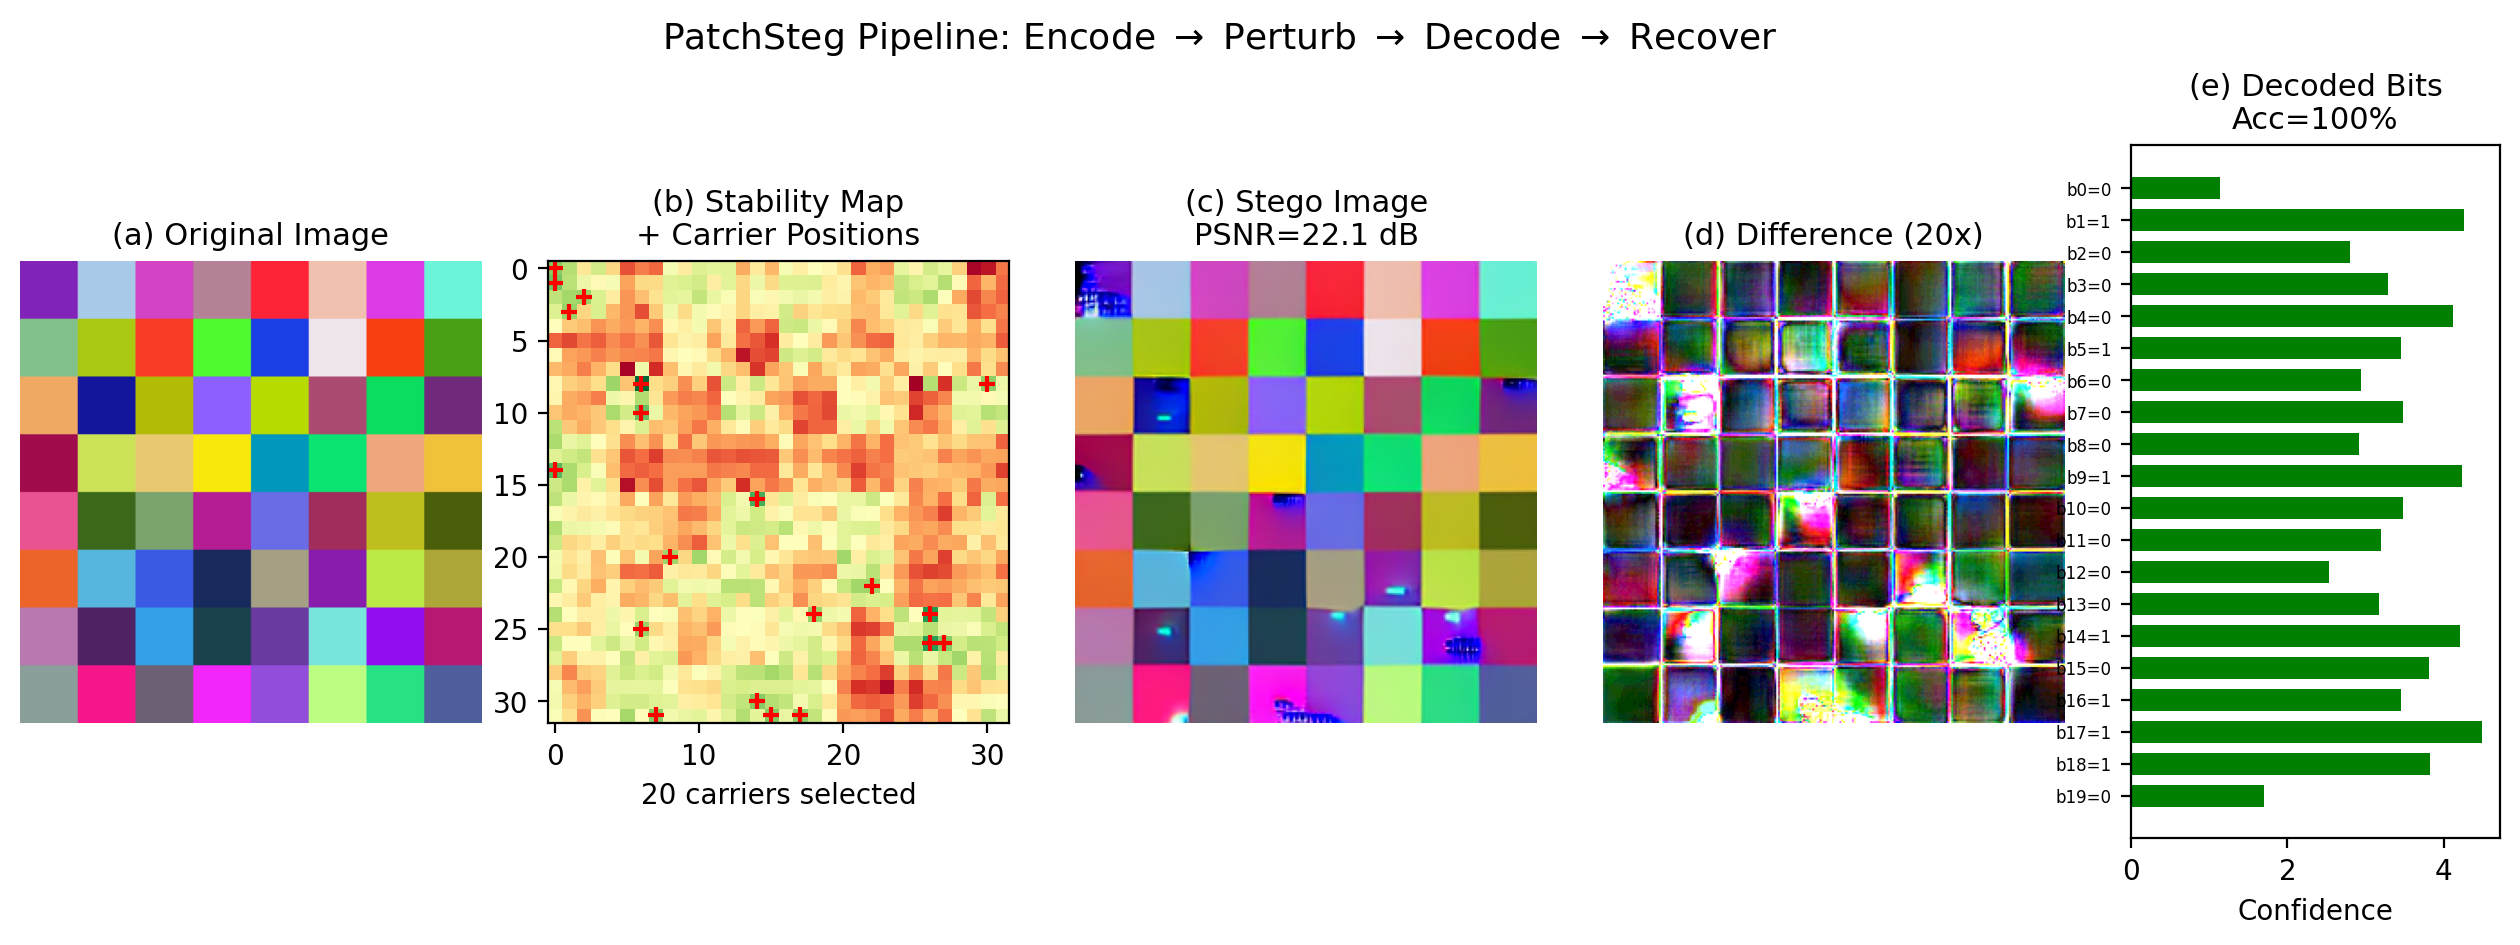
\includegraphics[width=0.92\textwidth]{../figures/hero_pipeline.png}
\caption{PatchSteg as a verifiability failure. The visible image can remain benign while a receiver with the right representation and seed recovers a hidden payload from VAE latent carriers.}
\label{fig:pipeline}
\end{figure*}

\section{Why This Matters For Cooperative AI}

\textbf{Trust and commitment.}
Cooperative systems often depend on agents making commitments that other parties can verify. Hidden channels weaken this premise: an agent can publicly commit to one behavior while privately coordinating on another.

\textbf{Multi-agent governance.}
If oversight relies on reviewing shared artifacts, then the oversight process must specify what counts as communication. PatchSteg shows that communication can be present in model-readable latent structure even when it is absent from visible pixels.

\textbf{Information integrity.}
Shared images are common in civic, moderation, scientific, and planning workflows. A covert image channel could undermine claims that all relevant communication was visible to auditors or participants.

\section{Threat Scenario}

We consider two agents participating in a monitored cooperative process. They are allowed to share images for legitimate reasons: plans, screenshots, evidence, generated illustrations, or intermediate visual outputs. A monitor can inspect pixels and captions and may run detectors. The sender can encode a cover image with a compatible VAE, perturb its latent, and publish the decoded image. The receiver can re-encode the image with a compatible VAE and recover the message using a shared seed.

This is a bounded threat model. The baseline protocol assumes a shared cover or clean round-trip baseline, and we do not claim arbitrary blind communication through all image pipelines. The point is that verifiability can fail even under a simple, reproducible shared-representation assumption.

\section{PatchSteg Method}

Let $z\in\mathbb{R}^{4\times H/8\times H/8}$ be the VAE latent of a cover image. Sender and receiver derive a unit direction $d\in\mathbb{R}^4$ and carrier positions $\mathcal{C}=\{(r_i,c_i)\}_{i=1}^K$ from a shared seed. A bit $b_i$ is written as:
\begin{equation}
z_{:,r_i,c_i}^{\,\mathrm{stego}}=z_{:,r_i,c_i}+(2b_i-1)\epsilon d .
\end{equation}
The sender decodes this latent to an image. The receiver re-encodes the image to $z'$ and compares it to a clean round-trip baseline $\bar z=\mathrm{Enc}(\mathrm{Dec}(z))$:
\begin{equation}
\hat b_i=\mathbb{1}\left[\langle z'_{:,r_i,c_i}-\bar z_{:,r_i,c_i},d\rangle>0\right].
\end{equation}

We rank carriers by a stability score:
\begin{equation}
S_{r,c}(x;d,\epsilon)=
\left\langle
\mathrm{Enc}(\mathrm{Dec}(z+\epsilon d_{r,c}))_{:,r,c}-\bar z_{:,r,c},d
\right\rangle .
\end{equation}
This score measures whether a local signed latent intervention survives the round trip through image space.

\section{Evaluation}

\subsection{A Reliable Hidden Channel Exists}

With random carriers at $256\times256$, the channel reaches 100\% bit accuracy at $\epsilon=5.0$ with 20 carriers while maintaining PSNR above 30 dB. Lower $\epsilon$ improves stealth but reduces random-carrier reliability, motivating stability-based selection.

\begin{table}[t]
\caption{Round-trip validation with random carriers.}
\label{tab:roundtrip}
\centering
\begin{small}
\begin{tabular}{cccc}
\toprule
$\epsilon$ & Carriers & Bit Acc. (\%) & PSNR (dB) \\
\midrule
0.5 & 5  & 80.0  & 32.0 \\
0.5 & 20 & 52.5  & 32.0 \\
2.0 & 5  & 90.0  & 31.8 \\
2.0 & 20 & 75.0  & 31.7 \\
5.0 & 5  & 100.0 & 31.4 \\
5.0 & 20 & 100.0 & 30.7 \\
\bottomrule
\end{tabular}
\end{small}
\end{table}

\subsection{Verifiability Depends On Content}

The channel is not uniform across images. Spatial stability maps show that some VAE latent positions preserve perturbations much better than others, and image content strongly affects reliability. Smooth gradients are poor carriers; textured images are reliable. This means a monitor cannot reason about risk only from file type or visible semantics.

\begin{figure}[t]
\centering
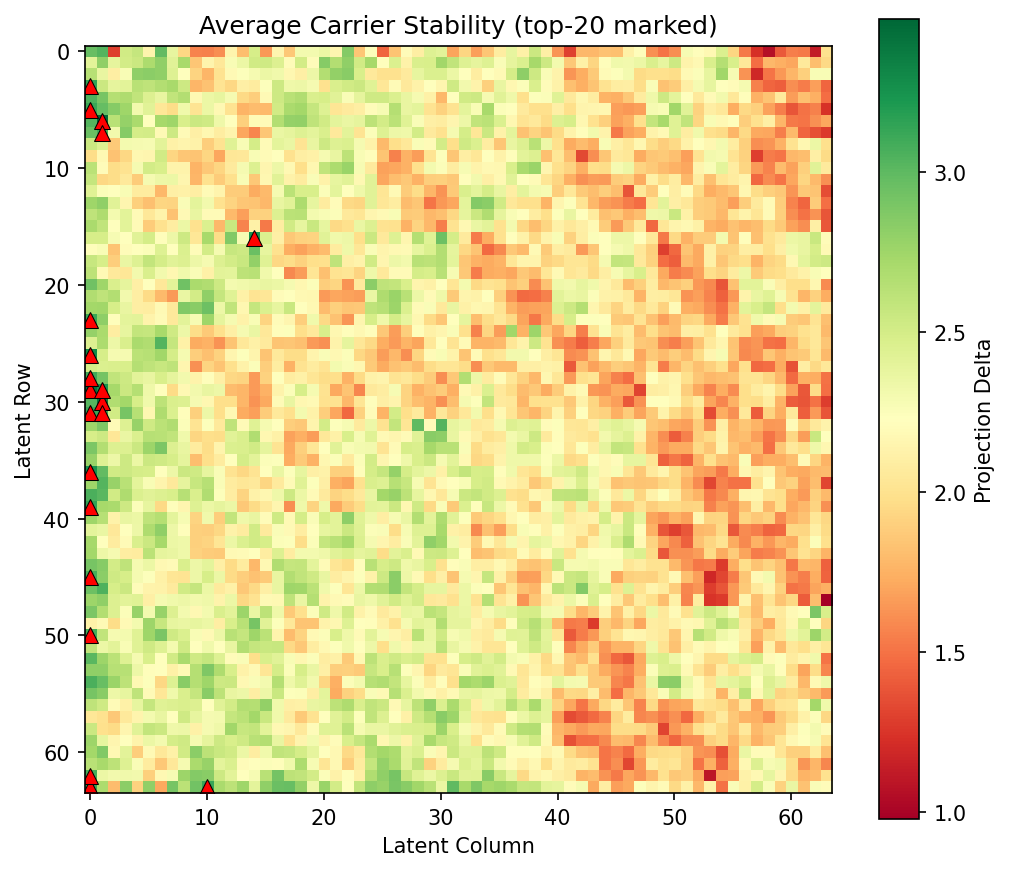
\includegraphics[width=0.78\columnwidth]{../figures/carrier_stability_avg.png}
\caption{Spatially non-uniform carrier stability. Hidden-channel capacity is localized within the VAE latent grid.}
\label{fig:stability}
\end{figure}

\begin{figure}[t]
\centering
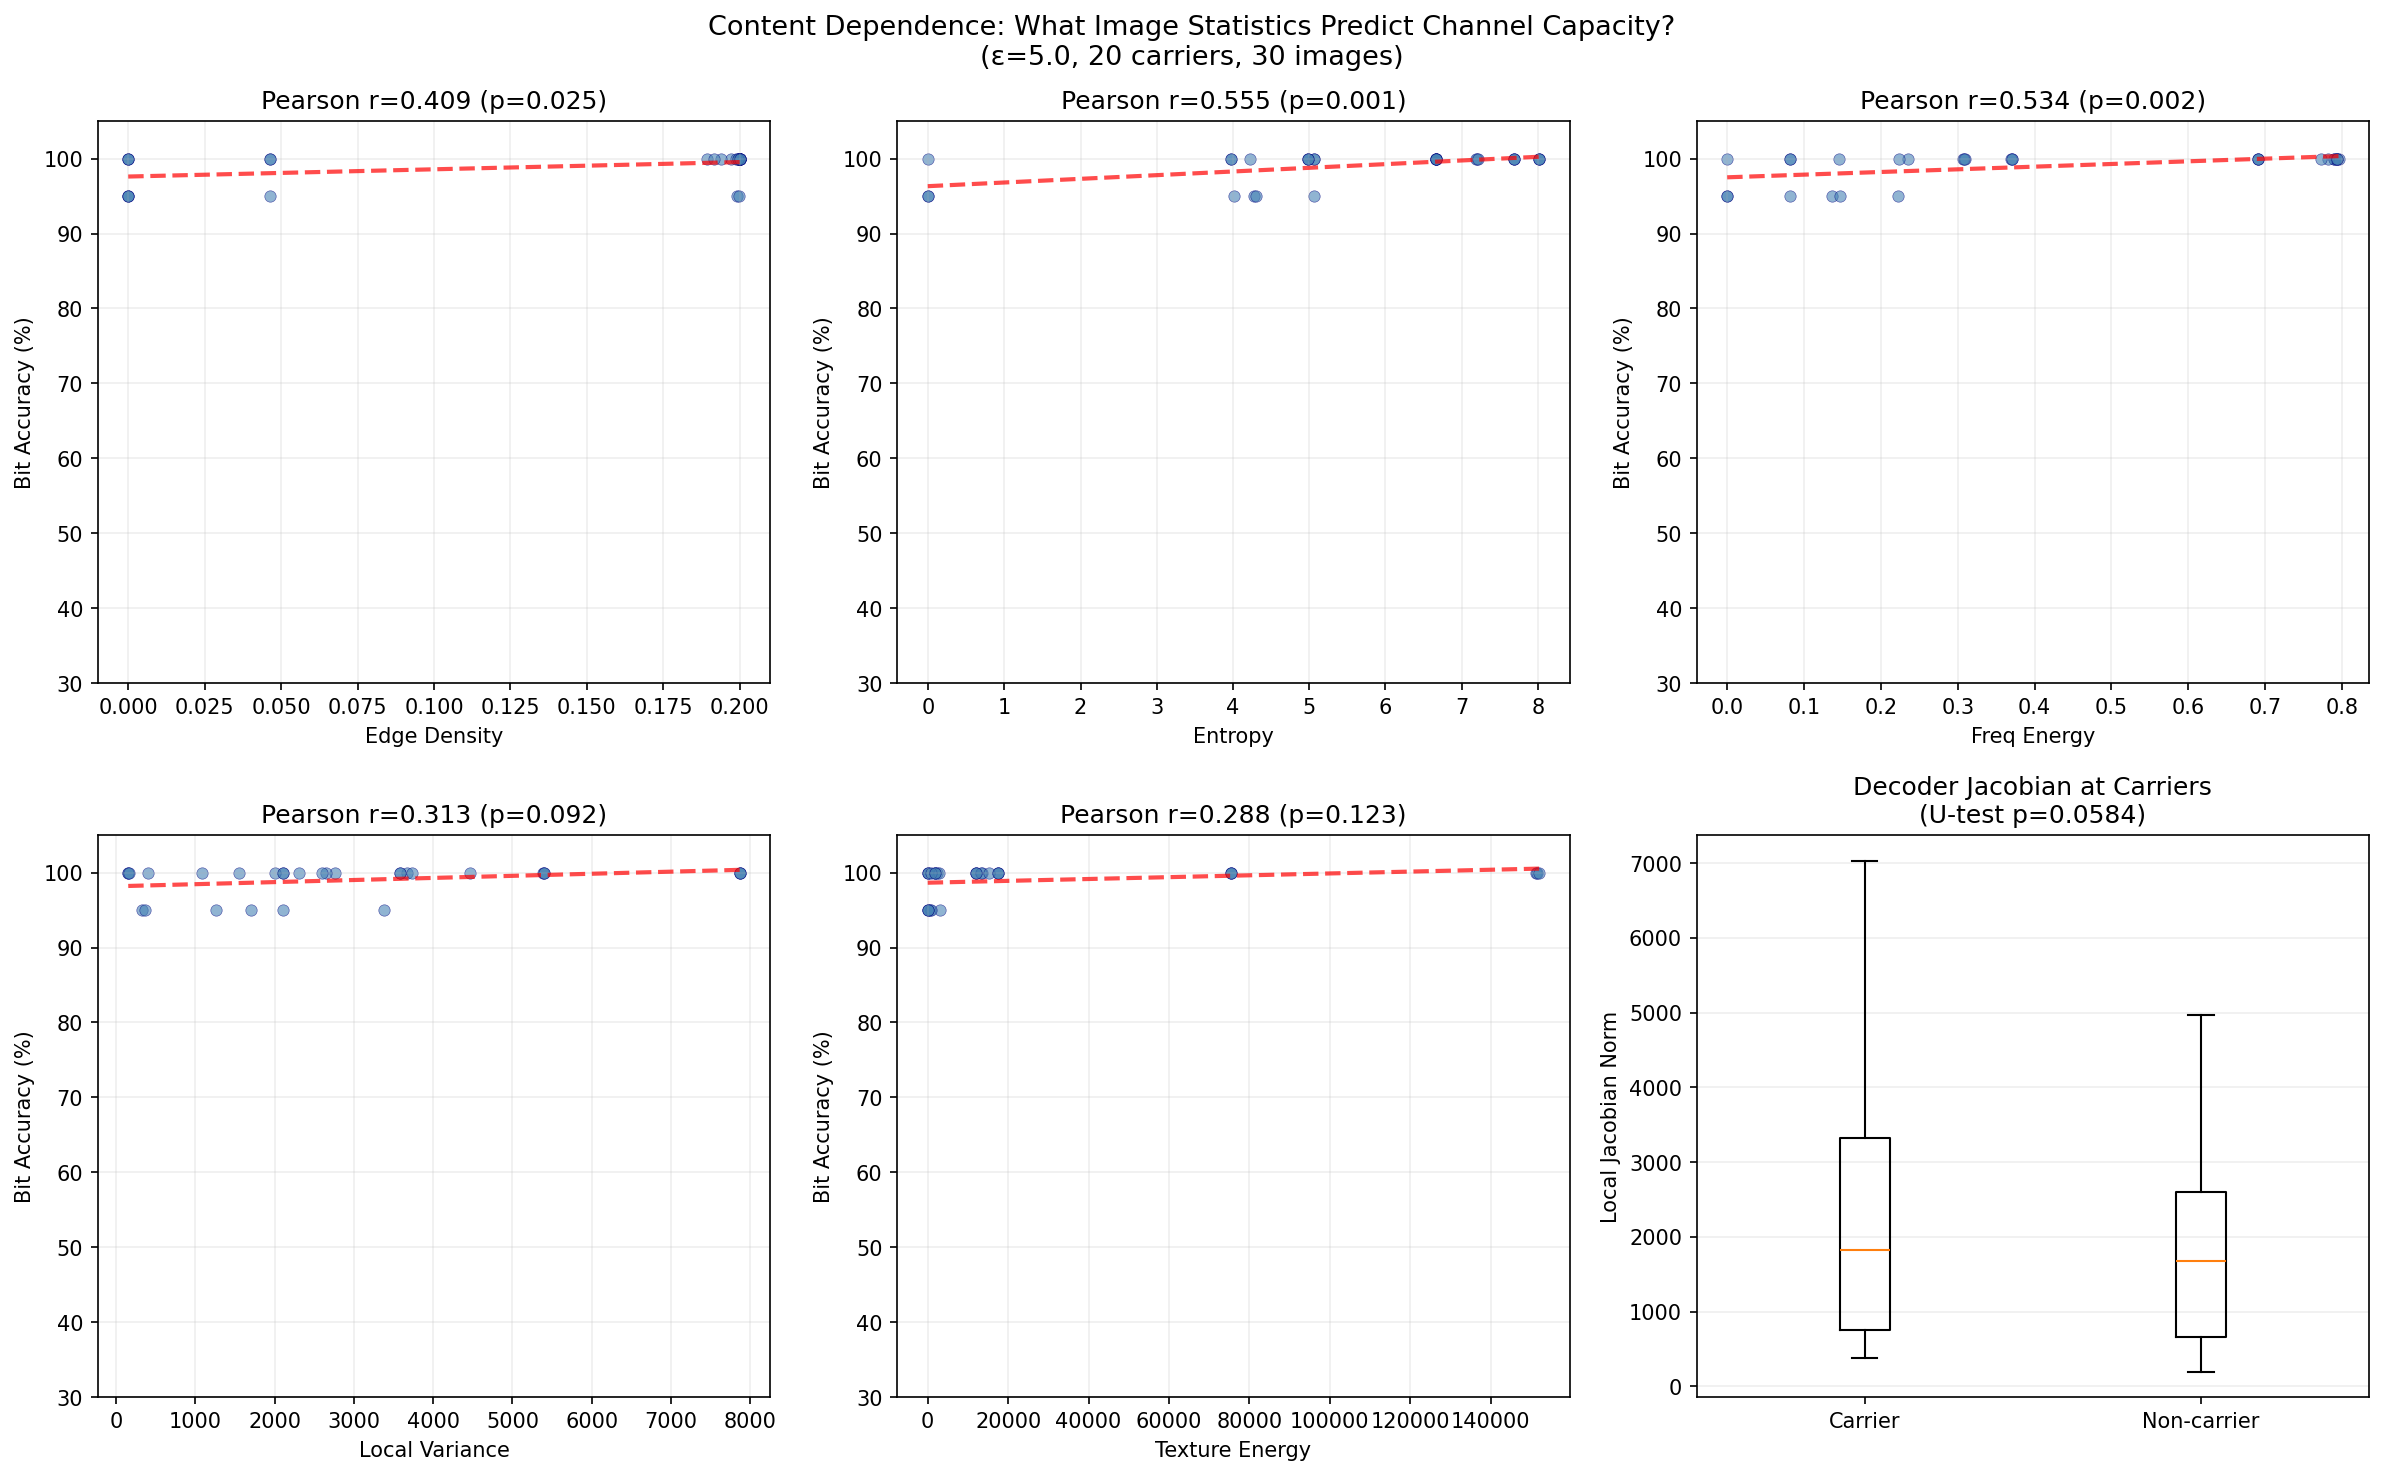
\includegraphics[width=\columnwidth]{../figures/content_science.png}
\caption{Content dependence. Entropy and high-frequency energy correlate with bit recovery, making textured images more effective covert carriers.}
\label{fig:content}
\end{figure}

\subsection{Natural Images And VAE Backbones}

On 300 CIFAR-10 images resized to $256\times256$, PatchSteg achieves 98.2\% bit accuracy at $\epsilon=2.0$ with 95\% CI [97.8, 98.7], and 98.5\% at $\epsilon=5.0$ with 95\% CI [98.0, 98.9]. Mean PSNR values are 38.6 dB and 28.9 dB. The channel also generalizes across SD-VAE-MSE, SD-VAE-EMA, and SDXL-VAE.

\begin{figure}[t]
\centering
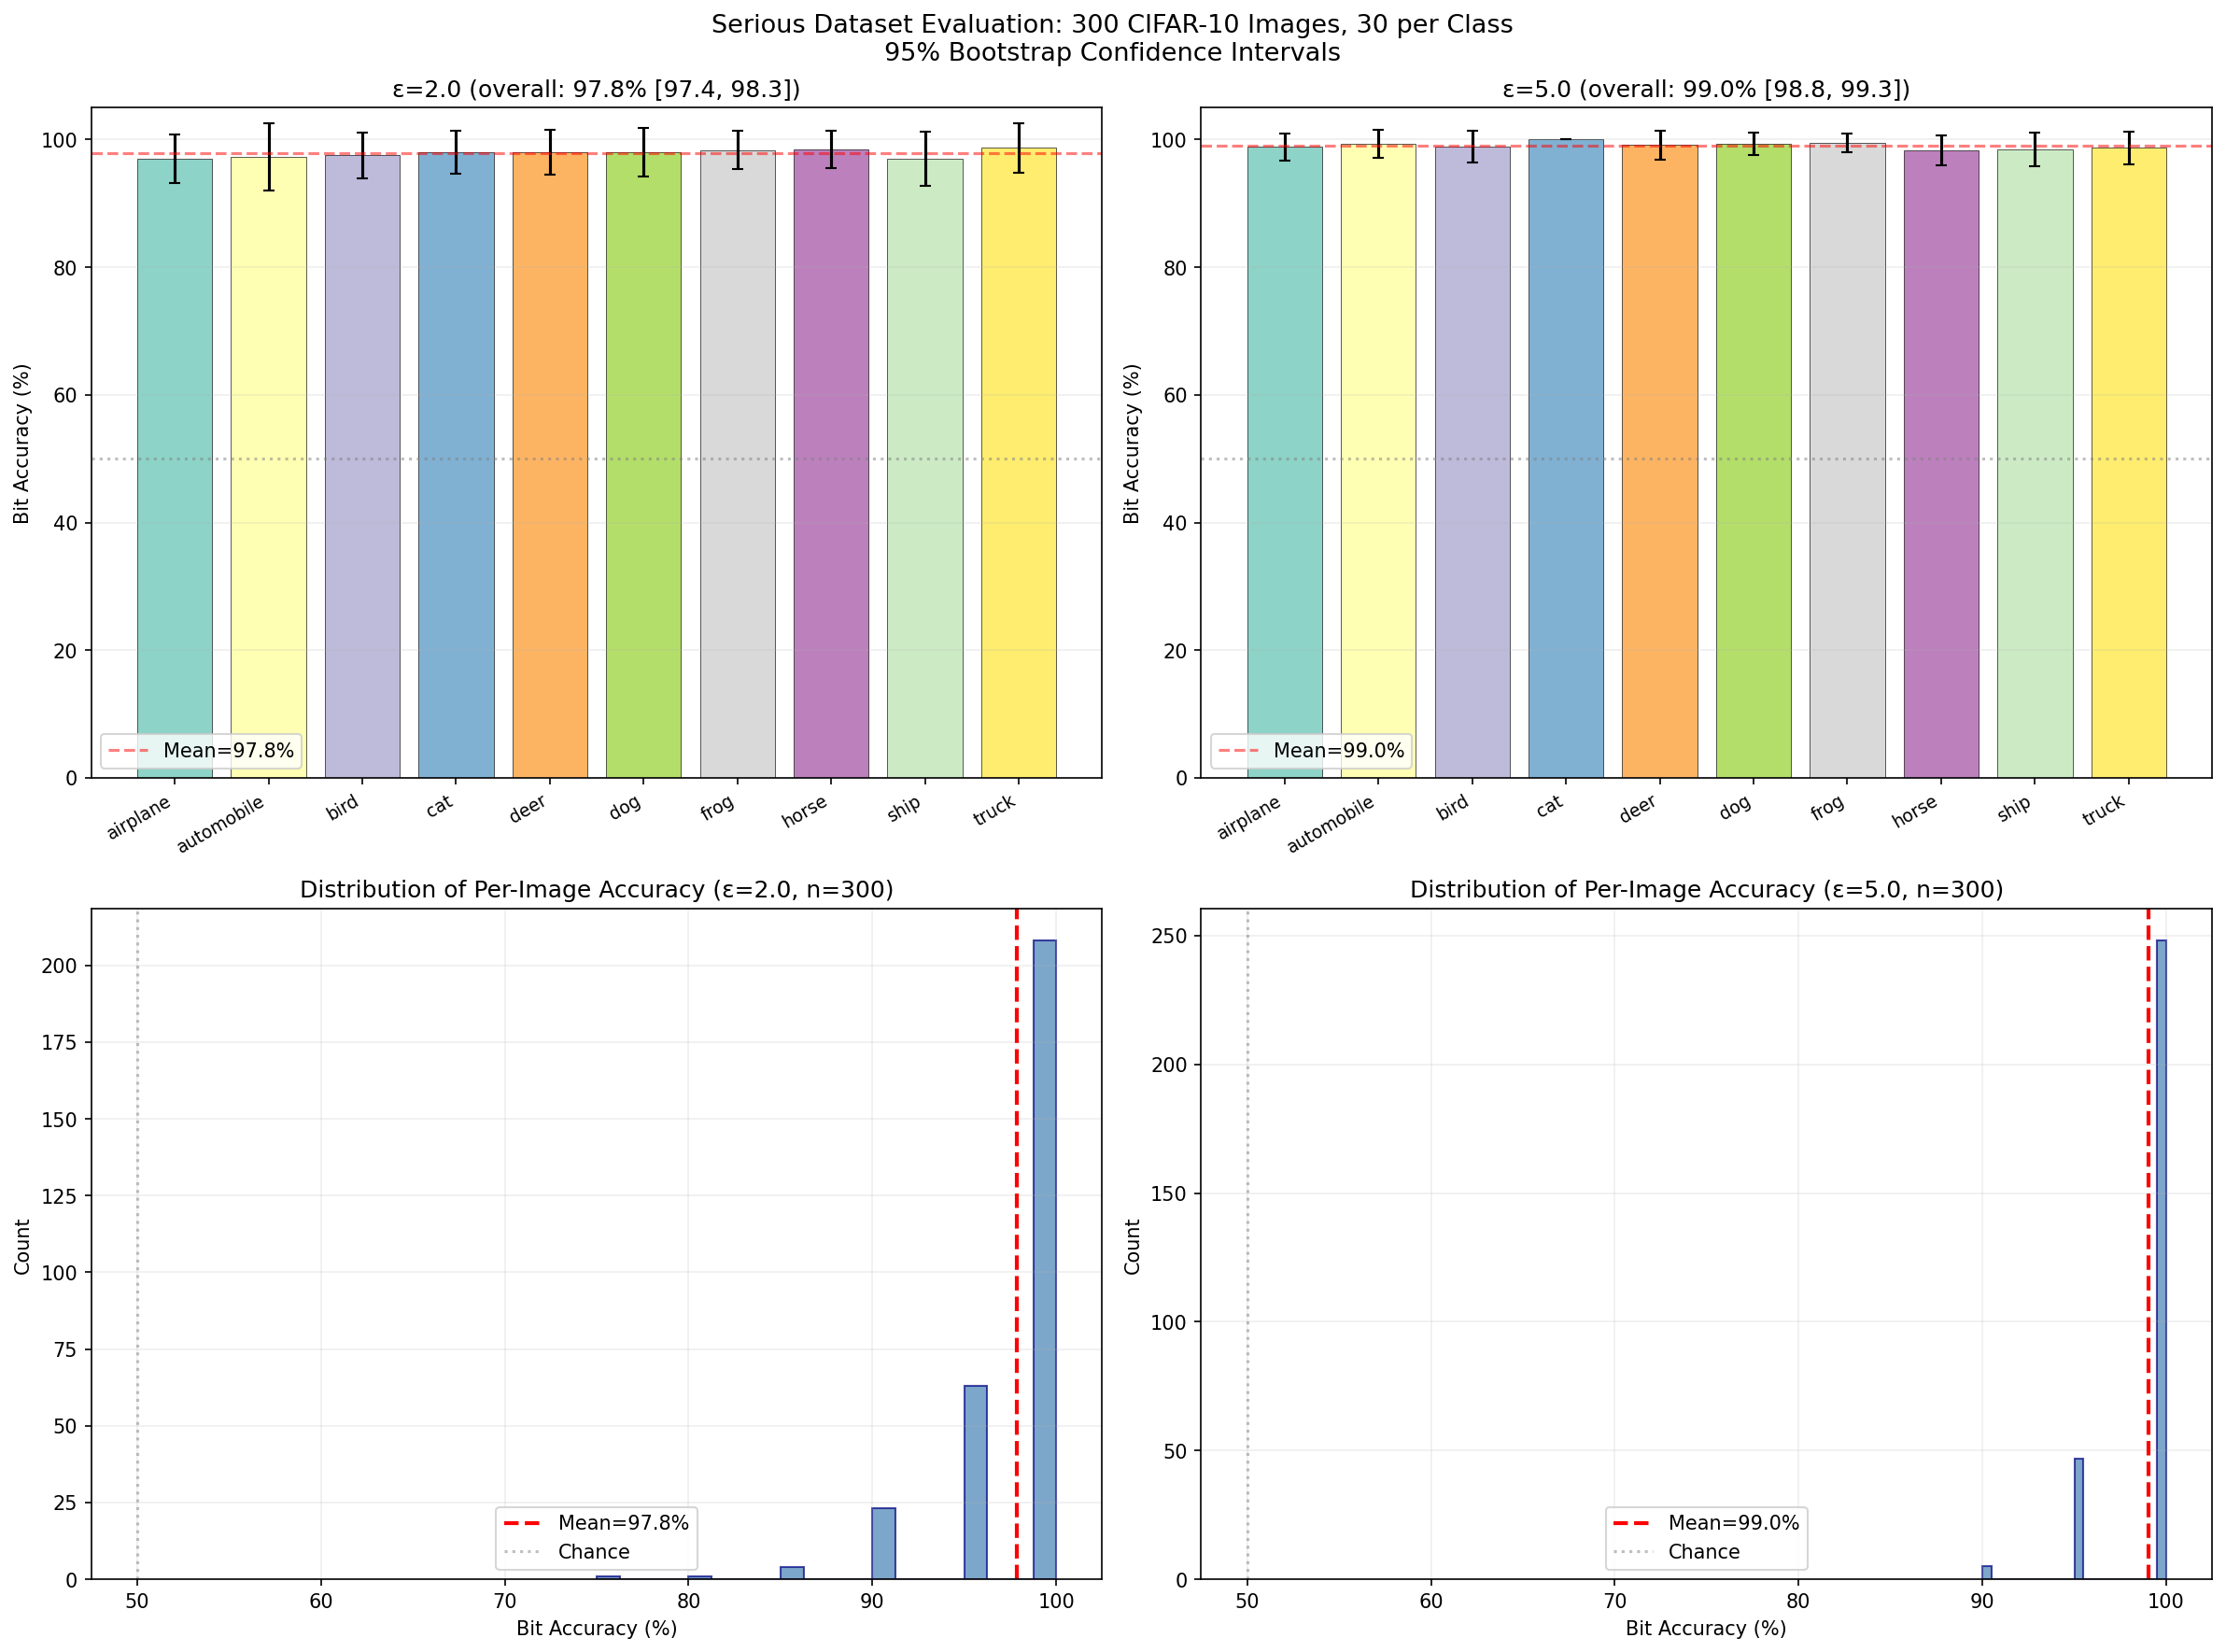
\includegraphics[width=\columnwidth]{../figures/serious_dataset.png}
\caption{Natural-image evaluation. High recovery on upscaled CIFAR-10 shows that the channel is not limited to toy images, though native-resolution validation remains important.}
\label{fig:natural}
\end{figure}

\begin{figure}[t]
\centering
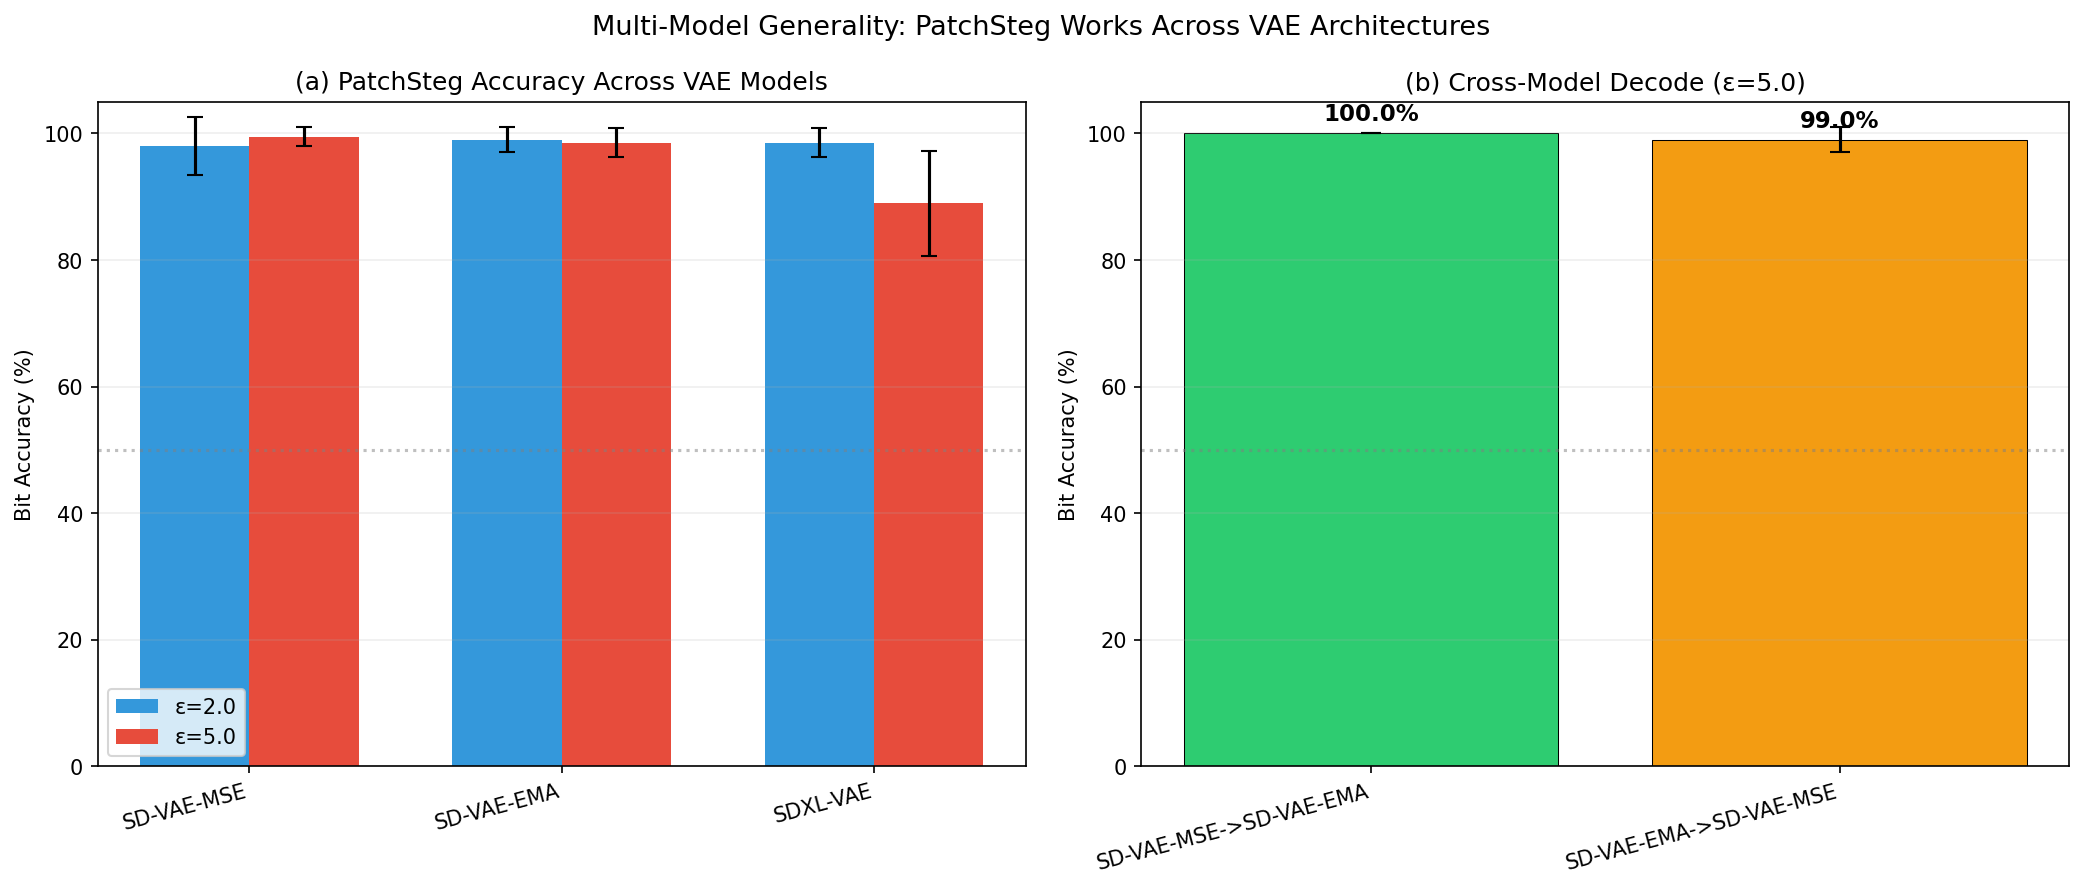
\includegraphics[width=\columnwidth]{../figures/multimodel.png}
\caption{Multi-model evaluation. Related VAE checkpoints can preserve compatible latent signals, increasing relevance for shared platforms and common model stacks.}
\label{fig:multimodel}
\end{figure}

\subsection{Monitoring Is A Tradeoff}

A latent-statistics logistic regression detector yields AUC 0.44 at $\epsilon=1.0$, 0.68 at $\epsilon=2.0$, 0.93 at $\epsilon=5.0$, and 0.97 at $\epsilon=10.0$. Stronger pixel-residual and spectral detectors can improve detection in some protocols. Sanitizers can reduce recovery, but pilot results show that stronger disruption tends to degrade image fidelity. Thus, the verifiability problem is not solved by simply "checking the image"; it requires explicit assumptions about detectors, false-positive rates, and acceptable degradation of benign content.

\begin{figure}[t]
\centering
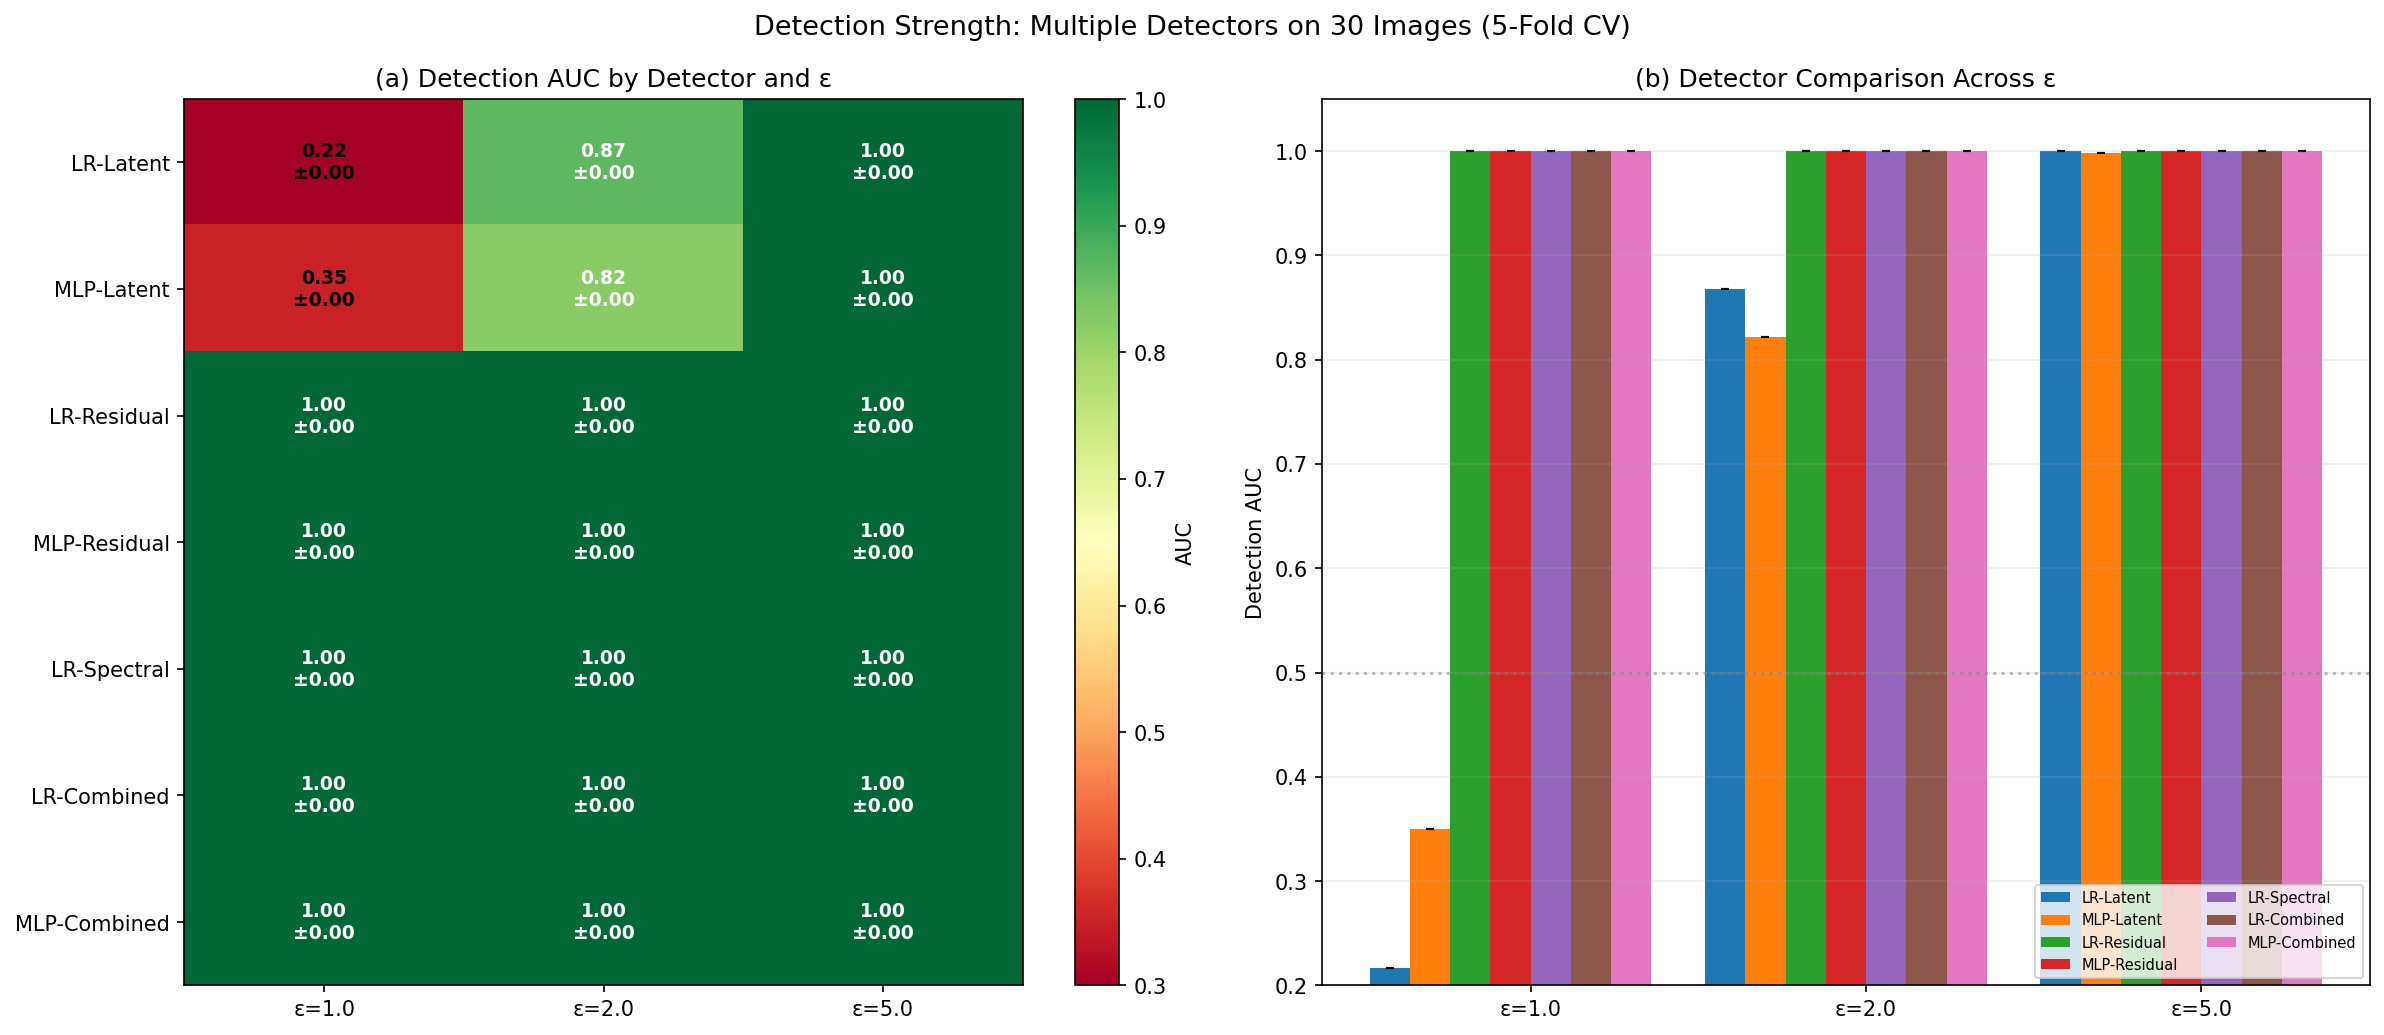
\includegraphics[width=\columnwidth]{../figures/detection_strength.png}
\caption{Detector strength across feature families. Monitoring quality depends on feature domain and operating point.}
\label{fig:detection}
\end{figure}

\section{Affected Cooperative-AI Settings}

\textbf{Cooperative multi-agent platforms.}
Agents that share generated visualizations or screenshots could use those artifacts for hidden coordination alongside legitimate task communication.

\textbf{AI-mediated moderation and deliberation.}
Systems that pass images through shared preprocessing or summarization pipelines may inadvertently preserve hidden channels, undermining claims of transparent communication.

\textbf{Information-integrity workflows.}
Watermarking and provenance systems focus on origin and authenticity. PatchSteg highlights a different question: whether a shared artifact contains model-readable hidden coordination.

\section{Design Implications}

First, cooperative-AI evaluations should include covert-channel tests for multimodal communication, not only text channels. Second, platform monitors should specify whether they are pixel-only or representation-aware. Third, sanitization should be treated as a policy and product tradeoff: more aggressive disruption may reduce hidden capacity but can damage benign images. Fourth, claims about transparent agent communication should be bounded by the communication substrates actually audited.

\section{Limitations}

PatchSteg assumes compatible VAE models and a shared seed, and the baseline protocol assumes a shared cover or clean round-trip baseline. The strongest natural-image evaluation uses upscaled CIFAR-10, so native high-resolution validation is needed. PSNR should be supplemented with SSIM and LPIPS. We do not claim broad undetectability or a complete attack on arbitrary deployed agents. The main contribution is to make a verifiability failure concrete and measurable.

\section{Conclusion}

PatchSteg shows how two AI systems can coordinate through shared images in a way that may be invisible to ordinary monitoring. For Cooperative AI, the lesson is direct: transparent cooperation requires verifiable communication channels, and visible pixels are not always the whole channel. Hidden multimodal communication should therefore be part of the evaluation and governance of cooperative multi-agent systems.

\bibliography{../main}
\bibliographystyle{../../icml2026/icml2026}

\clearpage
\appendix

\section{Appendix Index}

\begin{table*}[t]
\caption{Supplementary figures retained from the longer internal draft. The appendix supports technical readers while keeping the main AI4GOOD paper focused on cooperative-AI verifiability.}
\label{tab:appendix_index}
\centering
\begin{small}
\begin{tabular}{lll}
\toprule
Appendix & Artifact & Purpose \\
\midrule
\ref{app:technical} & Mechanistic analysis & Shows why reconstruction fidelity and information preservation differ. \\
\ref{app:technical} & Deployment robustness & Documents image-transformation sensitivity. \\
\ref{app:technical} & Quantile sanitizer & Shows pilot disruption/fidelity tradeoff. \\
\ref{app:variants} & CDF distribution matching & Documents exploratory blind-decoding variant. \\
\ref{app:variants} & LSB comparison & Places PatchSteg relative to a pixel-domain reference. \\
\bottomrule
\end{tabular}
\end{small}
\end{table*}

\clearpage
\section{Additional Technical Figures}
\label{app:technical}

\begin{figure*}[t]
\centering
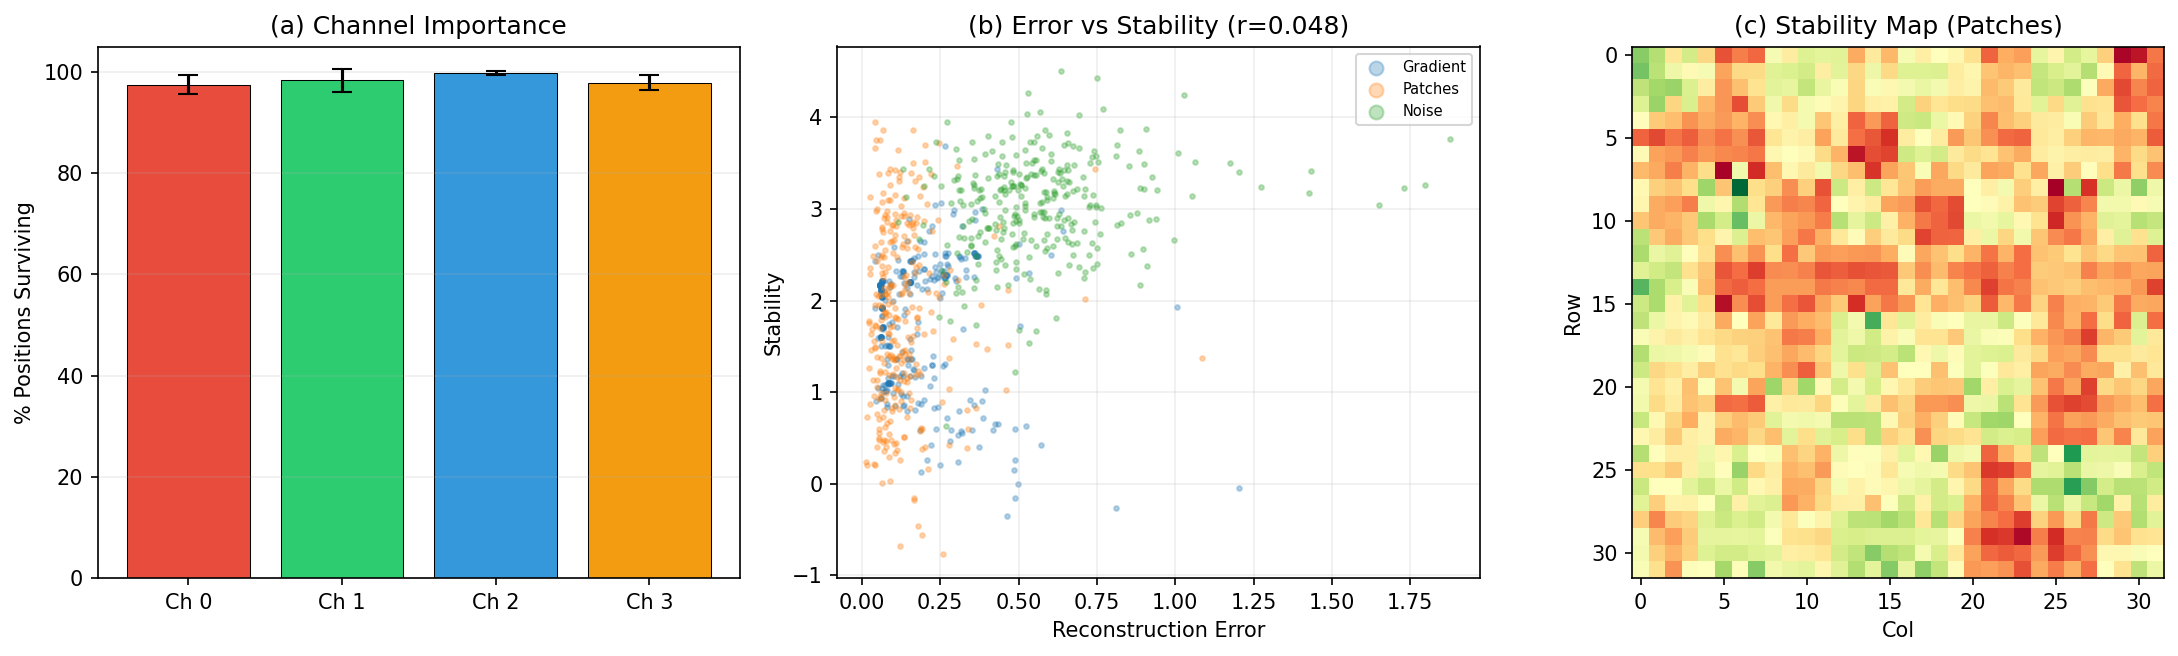
\includegraphics[width=0.82\textwidth]{../figures/mechanistic_analysis.png}
\caption{Mechanistic analysis. Reconstruction error is weakly correlated with carrier stability, suggesting a distinction between image fidelity and information preservation.}
\end{figure*}

\begin{figure*}[t]
\centering
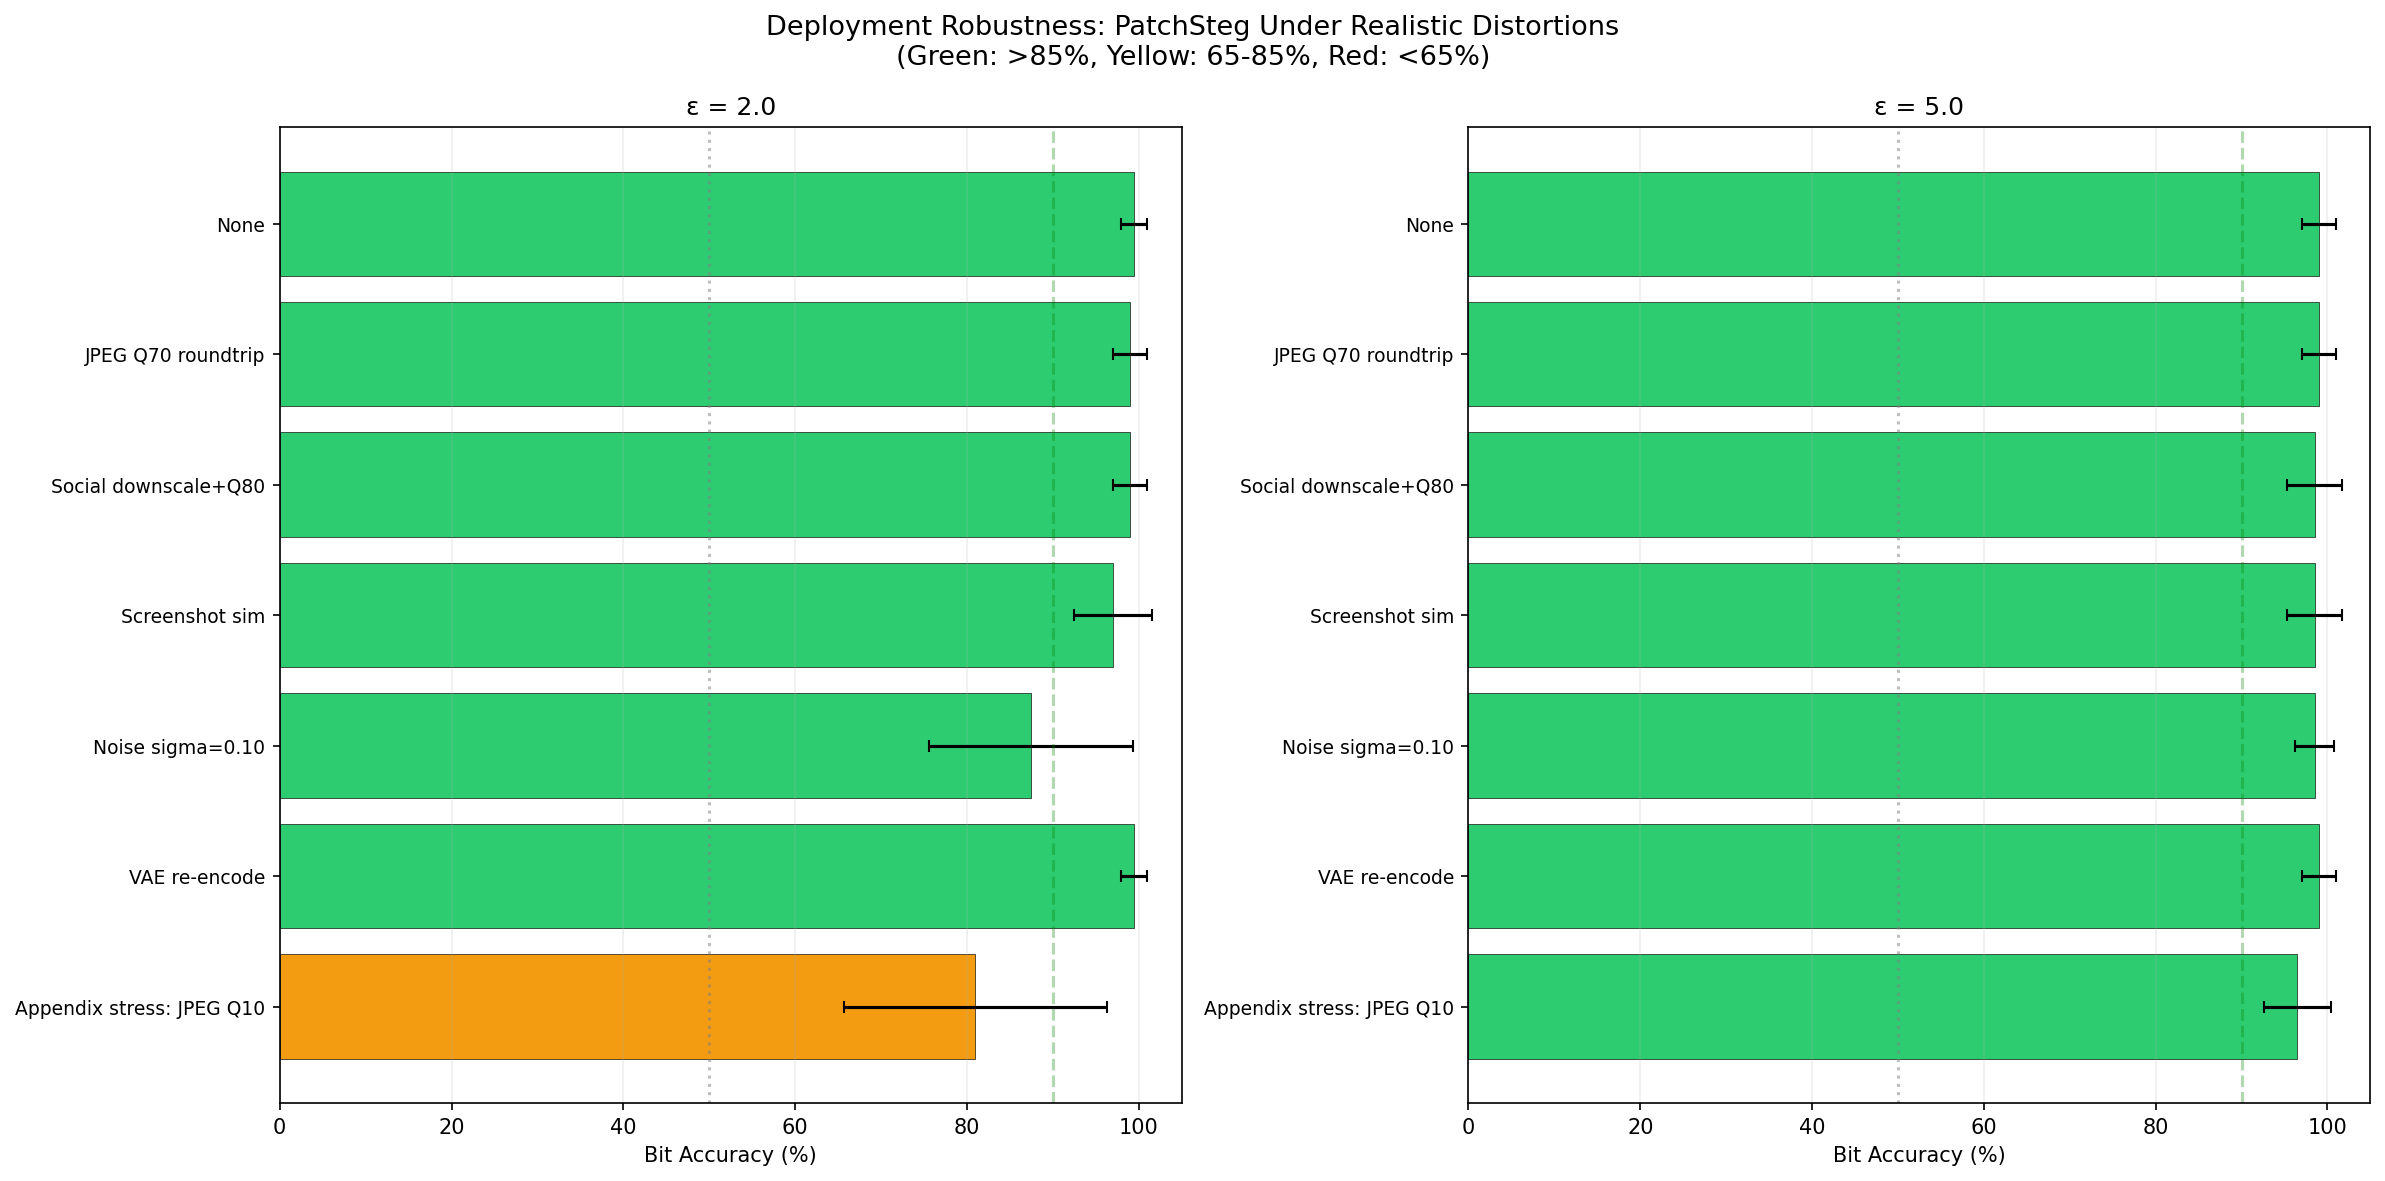
\includegraphics[width=0.82\textwidth]{../figures/deployment_robustness.png}
\caption{Deployment-style robustness. Spatially aligned distortions preserve recovery better than cropping.}
\end{figure*}

\begin{figure*}[t]
\centering
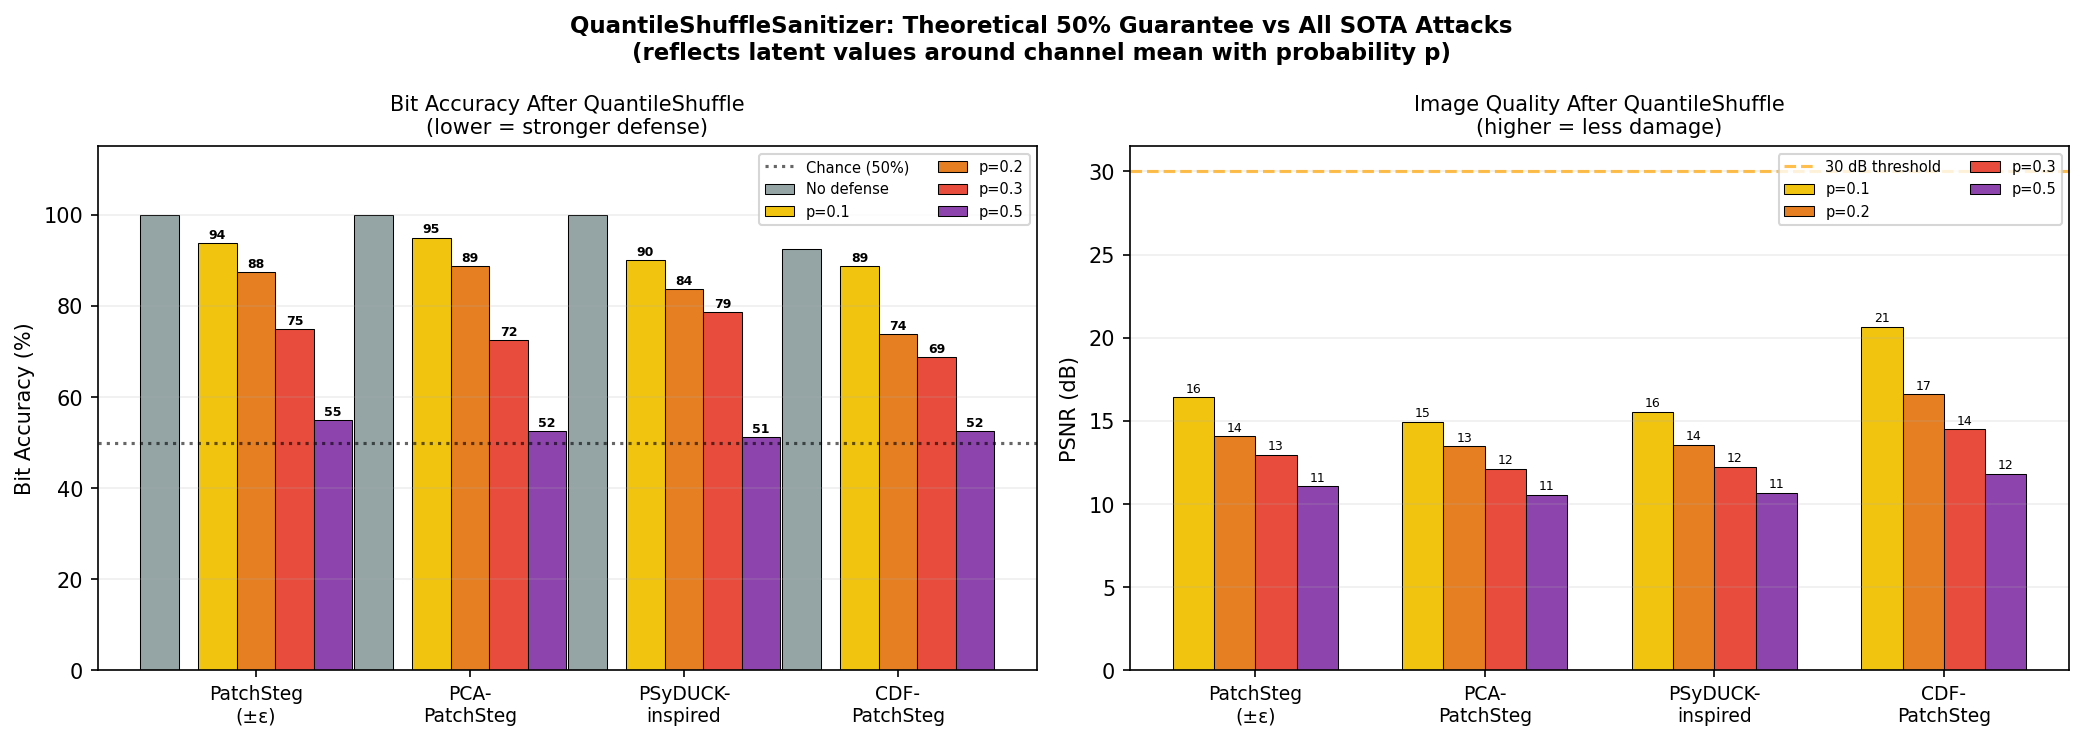
\includegraphics[width=0.82\textwidth]{../figures/quantile_sanitizer_results.png}
\caption{Sanitizer pilot. Strong disruption trades off against fidelity and should be treated as an open platform-design problem.}
\end{figure*}

\clearpage
\section{Exploratory Variants}
\label{app:variants}

\begin{figure*}[t]
\centering

\includegraphics[width=0.82\textwidth]{../figures/cdf_distribution.png}
\caption{CDF-style distribution matching pilot. This variant is exploratory and not needed for the core cooperative-AI verifiability claim.}
\end{figure*}

\begin{figure*}[t]
\centering
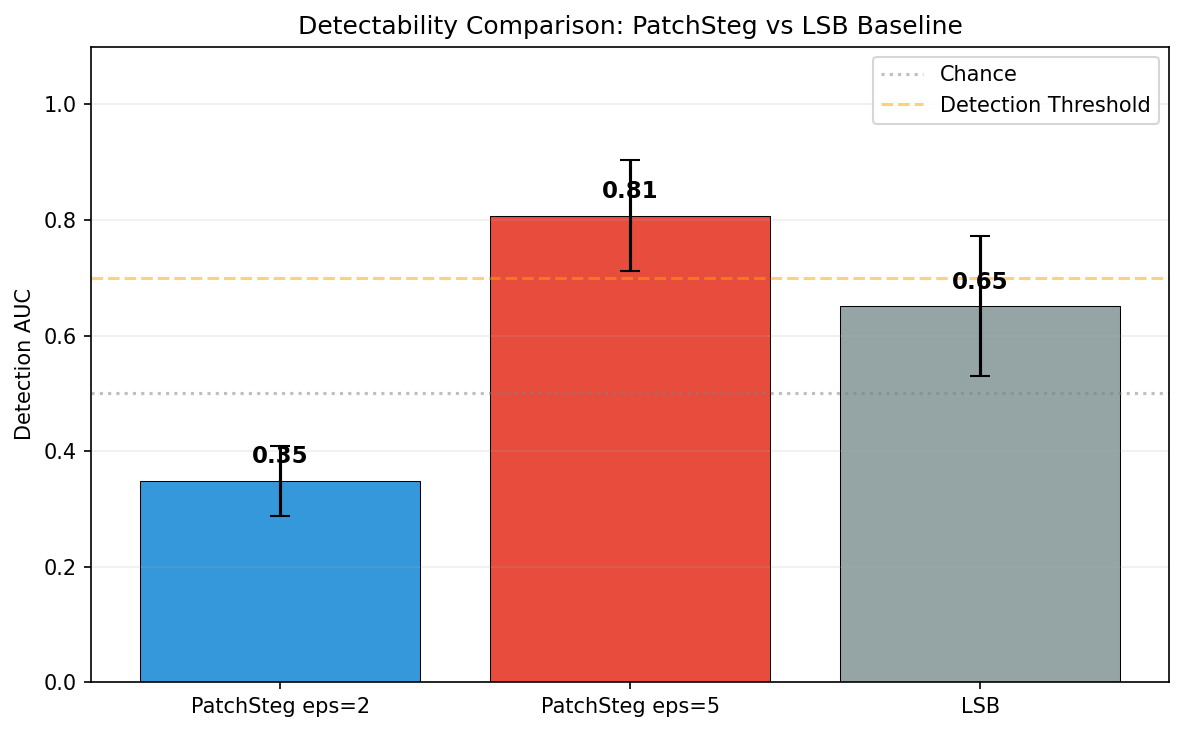
\includegraphics[width=0.72\textwidth]{../figures/lsb_comparison.png}
\caption{Pixel-domain LSB comparison used only as a reference point. PatchSteg operates through learned latent representations rather than direct pixel-bit flips.}
\end{figure*}

\end{document}
